\documentclass[tikz,border=1pt]{standalone} 
\usepackage{tikz}
% \usepackage{automata, arrows}
\usetikzlibrary{arrows.meta,calc,decorations.markings,math,arrows.meta}
\usetikzlibrary{positioning}
\begin{document}
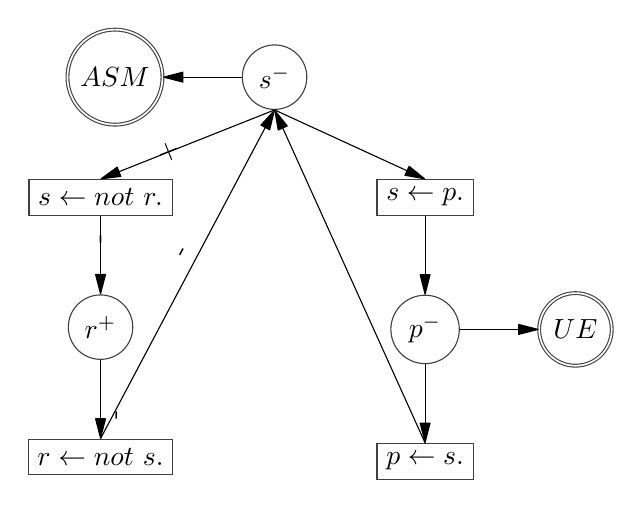
\begin{tikzpicture} [
    atom/.style={circle,  draw=black!75, minimum size=8mm},
    rule/.style={rectangle, draw=black!75, minimum size=3mm},
    sink/.style={circle, double, draw=black!75, minimum size=3mm},
    dummy/.style={midway,sloped,left},
    dummy2/.style={midway,sloped,left},
    >={Stealth[inset=0pt,length=8pt,angle'=28,round]}
    ]
    %Nodes

    \node[atom]      (s)       {$s^-$};
    \node[rule]      (rsp)  [below right=of s] {$s \leftarrow p.$};
    \node[rule]      (rsnotr)       [below left=of s] {$s \leftarrow not\ r.$};
    \node[atom]      (r)      [below =of rsnotr] {$r^+$};
    \node[rule]      (rrnots)  [below =of r] {$r \leftarrow not\ s.$};
    \node[atom]      (p)      [below =of rsp] {$p^-$};
    \node[rule]      (rps)  [below =of p] {$p \leftarrow s.$};
    \node[sink]      (asm)  [left =of s] {$ASM$};
    \node[sink]      (ue)  [right =of p] {$UE$};

    %Lines
    \draw[->] (s.south) -- (rsnotr.north) node[dummy] {+};
    \draw[->] (rsnotr.south) -- (r.north) node[dummy] {-};
    \draw[->] (r.south) -- (rrnots.north) node[dummy2, yshift=0.2cm, xshift=0.4cm] {-};
    \draw[->] (rrnots.north) -- (s.south) node[dummy2, yshift=0.2cm, xshift=0.4cm] {-};
    \draw[->]  (s.south)-- (rsp.north); node[dummy] {+};
    \draw[->]  (rsp.south)-- (p.north); node[dummy] {+};
    \draw[->]  (p.south)-- (rps.north);node[dummy] {+};
    \draw[->]  (rps.north)-- (s.south);node[dummy] {+};
    \draw[->]  (s.west)-- (asm.east); node[dummy] {-};
    \draw[->]  (p.east)-- (ue.west); node[dummy] {-};
\end{tikzpicture} 
\end{document}